% Blabla Matériel et Méthodes

In this part, will be detailed all the hardware, software and methods used to carry out simulations. 

\section{Hardware and Software}

    As this internship is 100\% digital, a good comuter is required. A personal computer (MacBook Air M1) as well as a computer provided by the laboratory (under Ubuntu) will be the main equipment for this internship. \medskip

    The main softwares are the following ones:

    \begin{enumerate}[\hspace{3em}$\bullet$]
        \item \textbf{Visual Studio Code (VS Code)}: a source-code editor developed by Microsoft.
        \item \textbf{Large-scale Atomic/Molecular Massively Parallel Simulator (LAMMPS)}: a molecular dynamics programm (coded in \verb|C++|) from \href{http://www.sandia.gov}{Sandia National Laboratories}.
        \item \textbf{Ovito}: a visualization and analysis software for output data generated in molecular dynamics. 
        \item \textbf{Perseus GRICAD}: high performance computing and storage platforms.  
    \end{enumerate}

    \subsection{LAMMPS}

        LAMMPS is an open-source molecular dynamic code with a focus on materials modeling. It provides potentials for solid-state materials (metals and semiconductors). It can be used to model atoms or, more generically, as a parallel particle simulator at the atomic, meso, or continuum scale. \medskip

        LAMMPS does not have any graphic interface which makes the handholding not that easy. The input code is written is \verb|.txt| files thats are compilled through a \verb|Makefile| called with a \verb|bash| command : \verb|lmp_serial -in input.file.txt|.
        
        LAMMPS provides a \verb|log.lammps| file as output. All the behaviour of the script (output values, warnings, errors \dots) is written in this file. However, with specific commands, this software can provide other outfile such as a \verb|dump.test| file, which will be useful to have a visualization of the material behaviour. \medskip

        Here is a quick recap : 

        \begin{center}
            \captionsetup{type=figure}
            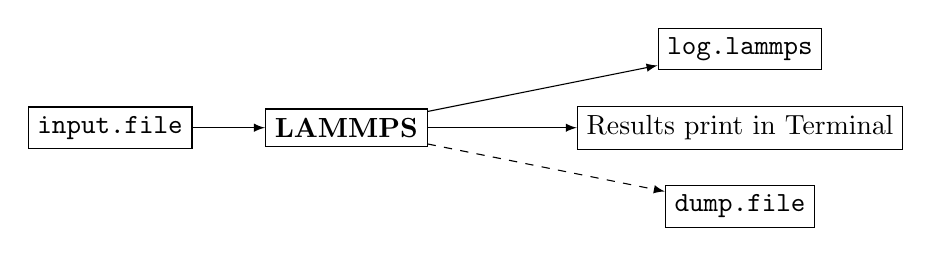
\begin{tikzpicture}
                \node[draw](I) at (0,0) {\verb|input.file|};
                \node[draw](L) at (3,0) {\textbf{LAMMPS}};
                \node[draw](LOG) at (8,1) {\verb|log.lammps|};
                \node[draw](RES) at (8,0) {Results print in Terminal};
                \node[draw](D) at (8,-1) {\verb|dump.file|};
                \draw[->,>=latex] (I) -- (L);
                \draw[->,>=latex] (L) -- (LOG);
                \draw[->,>=latex] (L) -- (RES);
                \draw[->,>=latex,dashed] (L) -- (D);
            \end{tikzpicture}
            \captionof{figure}{LAMMPS operation}
        \end{center}

    \subsection{Ovito}
        
        Ovito is a scientific visualization and data analysis tool for atomistic and other particle-based models. The community edition is free of charge under an open source license. Ovito has a Pro version which is a powerful extension with extended analysis toolset, visualization capabilities and automation with the \verb|Python| integration. For this intership, the community edition is used. \medskip

        Ovito will be used to visualize the behaviour of the atoms (mainly their position and velocity along the x,y and z axes). It will help to have a first sight of the simulation to see if there is no inconsitent behaviours before going deeper in the process.

        The visualization is based on the \verb|dump.file| that LAMMPS is producing. So here is the final scheme : 

        \begin{center}
            \captionsetup{type=figure}
            \begin{tikzpicture}
                \node[draw](I) at (0,0) {\verb|input.file|};
                \node[draw](L) at (3,0) {\textbf{LAMMPS}};
                \node[draw](LOG) at (8,1) {\verb|log.lammps|};
                \node[draw](RES) at (8,0) {Results print in Terminal};
                \node[draw](D) at (8,-1) {\verb|dump.file|};
                \node[draw](O) at (8,-2) {\textbf{Ovito}};
                \node[draw](OEX) at (5,-4) {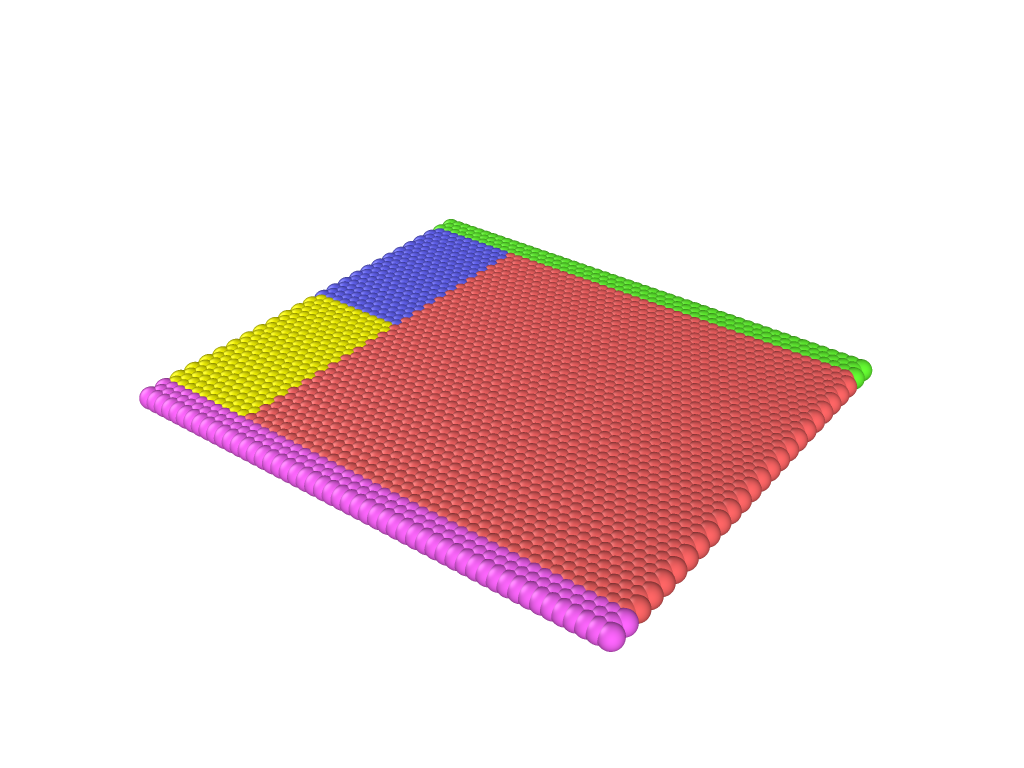
\includegraphics[scale = 0.1]{ovito_ex.png}};
                \draw[->,>=latex] (I) -- (L);
                \draw[->,>=latex] (L) -- (LOG);
                \draw[->,>=latex] (L) -- (RES);
                \draw[->,>=latex,dashed] (L) -- (D);
                \draw[->,>=latex] (D) -- (O);
                \draw[->,>=latex] (O) -| (OEX);
            \end{tikzpicture}
            \captionof{figure}{Final Operation Scheme}
        \end{center}
    
    \subsection{Perseus GRICAD}

        GRICAD offers intensive computing and data processing infrstructures to answer the needs of scientists. This tool provides an access to computing, grid, cloud, notebook and associated storage platforms. Moreover, an user support with assitance is opened. These infrastructures are open to all members of the scientific communities of the Grenoble site, as well as to their external collaborators. To have an access to this computing tool, a Perseus account is required. Once the Perseus account is created, you need to be member of the project to run your scripts. For this internship, the project is \verb|pr-atosimul|. \medskip

        GRICAD provides four computing culsters that are different (each cluster have their own hardware and configuration). Cluster access is normally done using a \verb|SSH Client| (Secure Shell Protocol) \cite{1}. However, SSH servers are vulnerable to scans and attacks so, for security reasons, it is not possible to let the clusters be directly accessed from the internet. GRICAD provides two SSH gateways that are more secure than the clusters. So the login method is to first, login to an SSH gateway and the login to the targeted cluster : 

        \begin{center}
            \captionsetup{type=figure}
            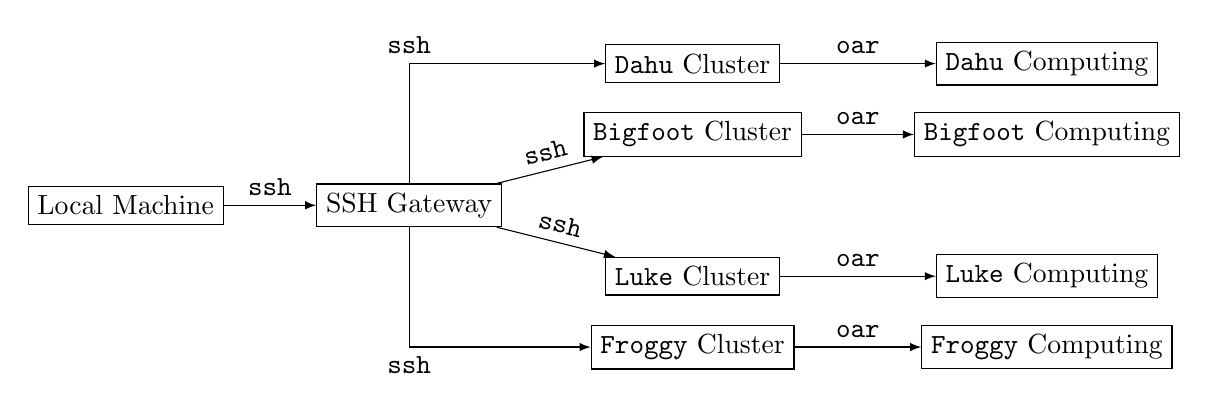
\begin{tikzpicture}[scale = 0.9]
                \node[draw](LOC) at (0,0) {Local Machine};
                \node[draw](SSH) at (4,0) {SSH Gateway};
                \node[draw](DAHU) at (8,2) {\verb|Dahu| Cluster};
                \node[draw](BIGF) at (8,1) {\verb|Bigfoot| Cluster};
                \node[draw](LUKE) at (8,-1) {\verb|Luke| Cluster};
                \node[draw](FROG) at (8,-2) {\verb|Froggy| Cluster};
                \node[draw](DAHUC) at (13,2) {\verb|Dahu| Computing};
                \node[draw](BIGFC) at (13,1) {\verb|Bigfoot| Computing};
                \node[draw](LUKEC) at (13,-1) {\verb|Luke| Computing};
                \node[draw](FROGC) at (13,-2) {\verb|Froggy| Computing};
                \draw[->,>=latex] (LOC) -- (SSH) node[midway,above]{\verb|ssh|};
                \draw[->,>=latex] (SSH) |- (DAHU) node[midway,above,sloped]{\verb|ssh|};
                \draw[->,>=latex] (SSH) -- (BIGF) node[midway,above,sloped]{\verb|ssh|};
                \draw[->,>=latex] (SSH) -- (LUKE) node[midway,above,sloped]{\verb|ssh|};
                \draw[->,>=latex] (SSH) |- (FROG) node[midway,below,sloped]{\verb|ssh|};
                \draw[->,>=latex] (DAHU) -- (DAHUC) node[midway,above]{\verb|oar|};
                \draw[->,>=latex] (BIGF) -- (BIGFC) node[midway,above]{\verb|oar|};
                \draw[->,>=latex] (LUKE) -- (LUKEC) node[midway,above]{\verb|oar|};
                \draw[->,>=latex] (FROG) -- (FROGC) node[midway,above]{\verb|oar|};
            \end{tikzpicture}
            \captionof{figure}{SSH cluster access schema}
        \end{center}
        
        Those two SSH gateways (called \verb|Rotule| and \verb|Trinity|) are grouped under a single DNS : \verb|access-gricad.univ-grenoble-alpes.fr|. This allows for load balancing on these two machines. Moreover, if one server came to fail, the other one is still available for computing. 
        
        The submission work for computing is made through a \verb|run.oar| file. It is a \verb|bash| script that provides the number of nodes and cores of the processor wanted by the user, the walltime (max time of computing), the name of some output files and then commands to run external scripts. (AJOUTER SCRIPT EN ANNEXE)